\documentclass[11pt]{beamer} % setting the documentclass to beamer makes this a presentation instead of a text document
\usetheme{metropolis} % this uses the metropolis theme for the presentation; I like it!
\usepackage{fontspec}
\setmainfont{Fira Sans} % this font is easy to read on a beamer, and works well with metropolis

% general package imports
%\usepackage{polyglossia}
%\setdefaultlanguage{german}
\usepackage{amsmath, amsfonts, amssymb}
\usepackage{graphicx} % for coloured text

\author{Leon Rauschning}
\title{Example presentation using \LaTeX}
\subtitle{Created for the GumbelTalks}
%\institute{Example Institute}
\date{15/4/23}

% define short commands for common colours
\newcommand{\red}[1]{\textcolor{red}{#1}}
\newcommand{\gray}[1]{\textcolor{gray}{#1}}

% this is a useful way to give sources on presentation slides
% essentially, this defines a footnote without a footnote number, 
% and decreases the footnote counter afterwards.
% this is one example of how to customize LaTeX to your needs!
\newcommand\blfootnote[1]{
\begingroup
\renewcommand\thefootnote{}\footnote{#1}
\addtocounter{footnote}{-1}
\endgroup
}

\begin{document}

\begin{frame} % slides are environments, like equations or figures
	\maketitle % title slide
\end{frame}

\begin{frame}
	% Slides can contain any kind of LaTeX code!
	% floats should be avoided, though
	In \LaTeX, a presentation is not fundamentally different from a text document.
	Much the same syntax can be used for typesetting text or equations.\\
	For example, we can write
	$$e^{i\pi} + 1 = 0$$
	, with $e$ representing Euler's number, $i$ being the imaginary unit and $\pi$ being the ratio of a circle's diameter to its circumference, as usual.
\end{frame}

\begin{frame}{Example Slide} % Slide with title
	\centering
	\bf Slides can also have titles!\\
	$\Rightarrow$ \sf this is a great way to provide some structure to your talk!
\end{frame}

\begin{frame}{$\ldots$ or images!}
	\centering
	% slides can also contain images
	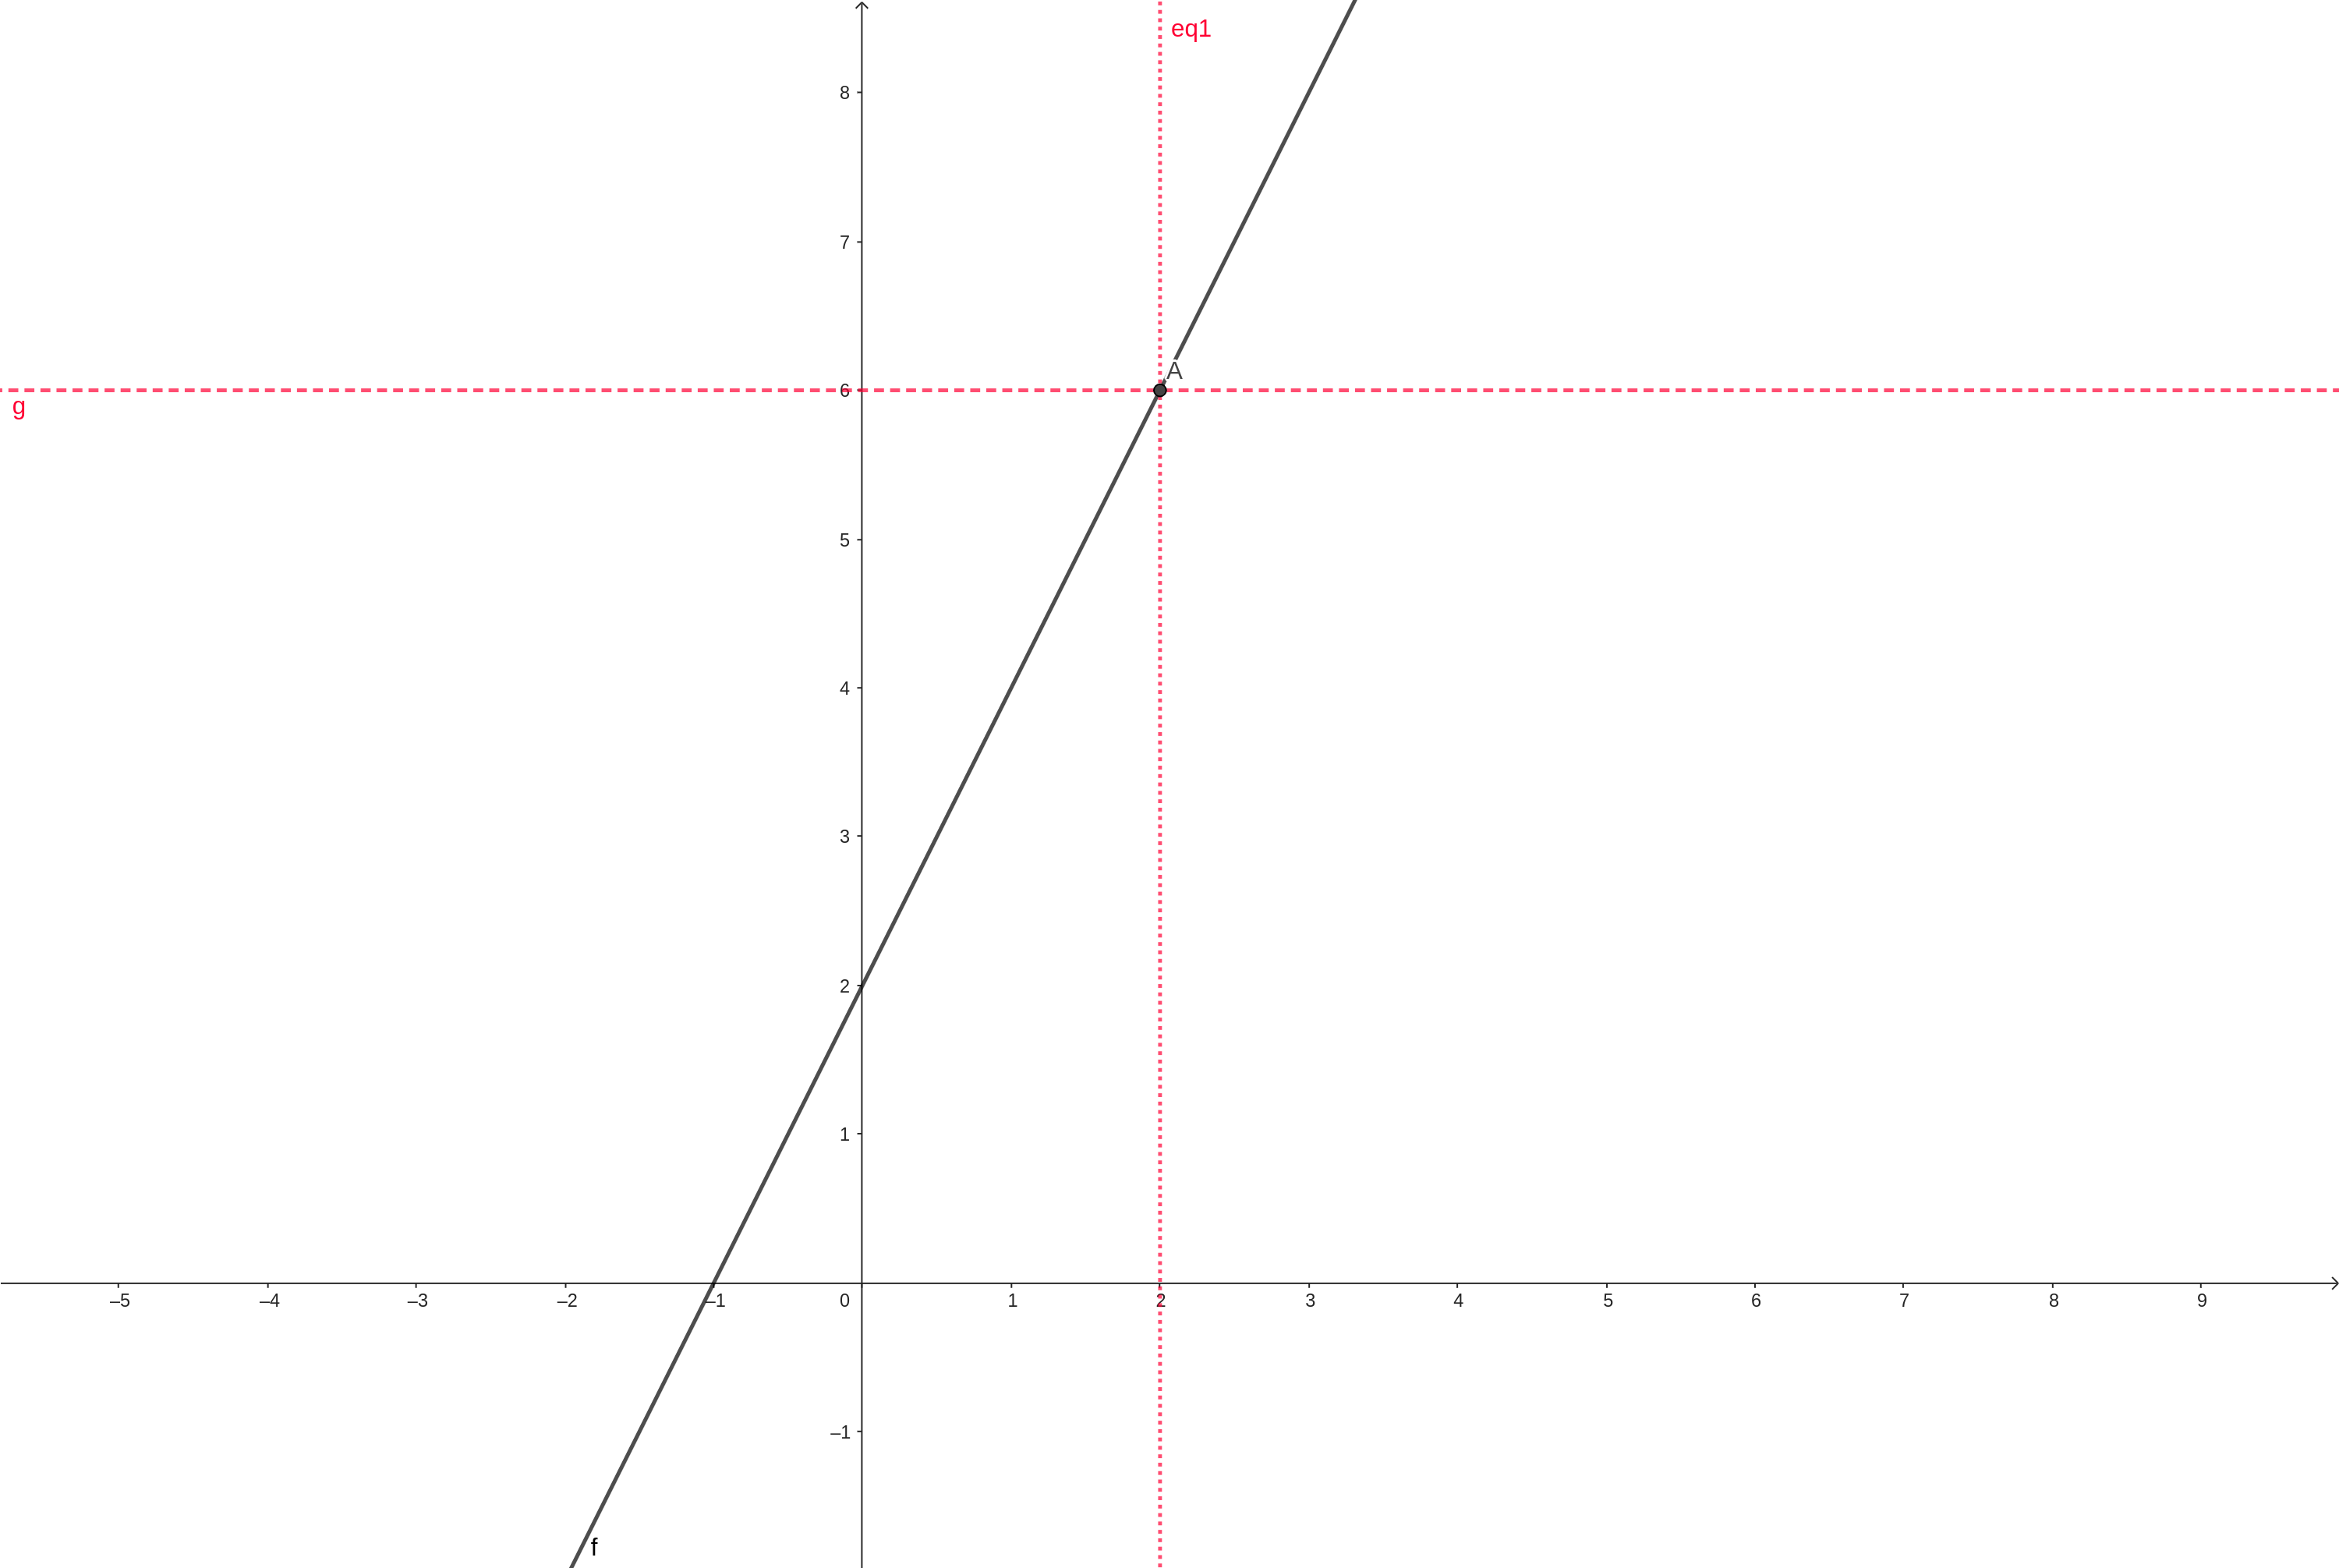
\includegraphics[width=.9\textwidth]{fig1-lineq.png} 
	\blfootnote{Image produced with GeoGebra} % give an image source using the command defined above 
\end{frame}

% you can also use sections and subsections etc. in presentations
\section*{Lists, Lists, Lists!} % suppress section numbering with a *
% I prefer unnumbered sections in presentations, but this is very much a matter of personal taste

\begin{frame}{Bullet points!}
	Bullet points are very useful for presentations. Advantages include:
	\begin{itemize} % these work the same as in a LaTeX document
		\item Less text
		\item easier to read
		\item[+] custom bullets!
	\end{itemize}
\end{frame}

\begin{frame}{Numbered Lists}
	\begin{enumerate}
		\item Number your list items automatically
		\item Easily insert new items or change the order
		\item \gray{???}
		\item \red{Profit!} % colouring text can also be a great visual tool!
	\end{enumerate}
\end{frame}

\section*{Animations}

\begin{frame}{Animations?}
	\centering
	\LaTeX cannot do swirly slide transitions, fade-ins or vibrating images$\ldots$\\[2\baselineskip] % have a double-width linebreak
	\pause % this renders everything up to it on an otherwise identical slide, and then continues rendering
	$\ldots$ but it can do overlays!\\
	\pause
	$\Rightarrow$ less flashy, but more flexible
\end{frame}

\begin{frame}{Overlays}
	\only<2->{\red{Complex}}
	\only<1>{Simple}
	overlays can add \only<2->{\red{or change}} content on a slide.\\
	\only<3->{
		And they work inside of any other Code!
		\begin{eqnarray*}
			H_n =& {\only<4>{\color{red}}\only<5>{\color{blue}}1} + {\only<4>{\color{red}}\frac{1}{2}} + {\only<5>{\color{blue}}\frac{1}{3}} + {\only<4>{\color{red}}\frac{1}{4}} +
			+ \frac{1}{5} + \frac{1}{6} + \frac{1}{7} + {\only<4>{\color{red}}\frac{1}{8}} + {\only<5>{\color{blue}}\frac{1}{9}} + 
			\frac{1}{10} + \frac{1}{11} + \cdots + \frac{1}{n}\\
	\end{eqnarray*}
	}
\end{frame}

\end{document}
